\documentclass[a4paper,12pt,openright]{book}
%\documentclass[a4paper, 12pt, openright, draft]{book}  Nalogo preverite tudi z opcijo draft, ki pokaže, katere vrstice so predolge! Pozor, v draft opciji, se slike ne pokažejo!
 
\usepackage[utf8]{inputenc}   % omogoča uporabo slovenskih črk kodiranih v formatu UTF-8
\usepackage[slovene,english]{babel}    % naloži, med drugim, slovenske delilne vzorce
\usepackage[pdftex]{graphicx}  % omogoča vlaganje slik različnih formatov
\usepackage{fancyhdr}          % poskrbi, na primer, za glave strani
\usepackage{amssymb}           % dodatni matematični simboli
\usepackage{amsmath}           % eqref, npr.
\usepackage{hyperxmp}
\usepackage[hyphens]{url}
\usepackage{csquotes}
\usepackage[pdftex, colorlinks=true,
						citecolor=black, filecolor=black, 
						linkcolor=black, urlcolor=black,
						pdfproducer={LaTeX}, pdfcreator={LaTeX}]{hyperref}

\usepackage{color}
\usepackage{soul}
\usepackage{tabularx}
\usepackage{listings}


\usepackage[
backend=biber,
style=numeric,
sorting=nty,
]{biblatex}


\addbibresource{literatura.bib} %Imports bibliography file


%%%%%%%%%%%%%%%%%%%%%%%%%%%%%%%%%%%%%%%%
%	DIPLOMA INFO
%%%%%%%%%%%%%%%%%%%%%%%%%%%%%%%%%%%%%%%%
\newcommand{\ttitle}{Generiranje slik staršev na podlagi slik otrok}
\newcommand{\ttitleEn}{Generation of parent images based on images of their children}
\newcommand{\tsubject}{\ttitle}
\newcommand{\tsubjectEn}{\ttitleEn}
\newcommand{\tauthor}{Vid Potočnik}
\newcommand{\tkeywords}{GAN, StyleGAN, PyTorch, ChildGAN, KinshipGAN, DNA-Net, Families In The Wild, linearna regresija, napovedni modeli, genetika}
\newcommand{\tkeywordsEn}{GAN, StyleGAN, PyTorch, ChildGAN, KinshipGAN, DNA-Net, Families In The Wild, linear regression, prediction models, genetics}

%%%%%%%%%%%%%%%%%%%%%%%%%%%%%%%%%%%%%%%%
%	HYPERREF SETUP
%%%%%%%%%%%%%%%%%%%%%%%%%%%%%%%%%%%%%%%%
\hypersetup{pdftitle={\ttitle}}
\hypersetup{pdfsubject=\ttitleEn}
\hypersetup{pdfauthor={\tauthor}}
\hypersetup{pdfkeywords=\tkeywordsEn}

%%%%%%%%%%%%%%%%%%%%%%%%%%%%%%%%%%%%%%%%
% postavitev strani
%%%%%%%%%%%%%%%%%%%%%%%%%%%%%%%%%%%%%%%%  

\addtolength{\marginparwidth}{-20pt} % robovi za tisk
\addtolength{\oddsidemargin}{40pt}
\addtolength{\evensidemargin}{-40pt}

\renewcommand{\baselinestretch}{1.3} % ustrezen razmik med vrsticami
\setlength{\headheight}{15pt}        % potreben prostor na vrhu
\renewcommand{\chaptermark}[1]%
{\markboth{\MakeUppercase{\thechapter.\ #1}}{}} \renewcommand{\sectionmark}[1]%
{\markright{\MakeUppercase{\thesection.\ #1}}} \renewcommand{\headrulewidth}{0.5pt} \renewcommand{\footrulewidth}{0pt}
\fancyhf{}
\fancyhead[LE,RO]{\sl \thepage} 
%\fancyhead[LO]{\sl \rightmark} \fancyhead[RE]{\sl \leftmark}
\fancyhead[RE]{\sc \tauthor}              % dodal Solina
\fancyhead[LO]{\sc Diplomska naloga}     % dodal Solina


\newcommand{\BibLaTeX}{{\sc Bib}\LaTeX}
\newcommand{\BibTeX}{{\sc Bib}\TeX}

%%%%%%%%%%%%%%%%%%%%%%%%%%%%%%%%%%%%%%%%
% naslovi
%%%%%%%%%%%%%%%%%%%%%%%%%%%%%%%%%%%%%%%%  

\newcommand{\autfont}{\Large}
\newcommand{\titfont}{\LARGE\bf}
\newcommand{\clearemptydoublepage}{\newpage{\pagestyle{empty}\cleardoublepage}}
\setcounter{tocdepth}{1}	      % globina kazala

%%%%%%%%%%%%%%%%%%%%%%%%%%%%%%%%%%%%%%%%
% konstrukti
%%%%%%%%%%%%%%%%%%%%%%%%%%%%%%%%%%%%%%%%  
\newtheorem{izrek}{Izrek}[chapter]
\newtheorem{trditev}{Trditev}[izrek]
\newenvironment{dokaz}{\emph{Dokaz.}\ }{\hspace{\fill}{$\Box$}}


%%%%%%%%%%%%%%%%%%%%%%%%%%%%%%%%%%%%%%%%%%%%%%%%%%%%%%%%%%%%%%%%%%%%%%%%%%%%%%%
%% PDF-A
%%%%%%%%%%%%%%%%%%%%%%%%%%%%%%%%%%%%%%%%%%%%%%%%%%%%%%%%%%%%%%%%%%%%%%%%%%%%%%%

%%%%%%%%%%%%%%%%%%%%%%%%%%%%%%%%%%%%%%%% 
% define medatata
%%%%%%%%%%%%%%%%%%%%%%%%%%%%%%%%%%%%%%%% 
\def\Title{\ttitle}
\def\Author{\tauthor, matjaz.kralj@fri.uni-lj.si}
\def\Subject{\ttitleEn}
\def\Keywords{\tkeywordsEn}

%%%%%%%%%%%%%%%%%%%%%%%%%%%%%%%%%%%%%%%% 
% \convertDate converts D:20080419103507+02'00' to 2008-04-19T10:35:07+02:00
%%%%%%%%%%%%%%%%%%%%%%%%%%%%%%%%%%%%%%%% 
\def\convertDate{%
    \getYear
}

{\catcode`\D=12
 \gdef\getYear D:#1#2#3#4{\edef\xYear{#1#2#3#4}\getMonth}
}
\def\getMonth#1#2{\edef\xMonth{#1#2}\getDay}
\def\getDay#1#2{\edef\xDay{#1#2}\getHour}
\def\getHour#1#2{\edef\xHour{#1#2}\getMin}
\def\getMin#1#2{\edef\xMin{#1#2}\getSec}
\def\getSec#1#2{\edef\xSec{#1#2}\getTZh}
\def\getTZh +#1#2{\edef\xTZh{#1#2}\getTZm}
\def\getTZm '#1#2'{%
    \edef\xTZm{#1#2}%
    \edef\convDate{\xYear-\xMonth-\xDay T\xHour:\xMin:\xSec+\xTZh:\xTZm}%
}

%\expandafter\convertDate\pdfcreationdate 

%%%%%%%%%%%%%%%%%%%%%%%%%%%%%%%%%%%%%%%%
% get pdftex version string
%%%%%%%%%%%%%%%%%%%%%%%%%%%%%%%%%%%%%%%% 
\newcount\countA
\countA=\pdftexversion
\advance \countA by -100
\def\pdftexVersionStr{pdfTeX-1.\the\countA.\pdftexrevision}


%%%%%%%%%%%%%%%%%%%%%%%%%%%%%%%%%%%%%%%%
% XMP data
%%%%%%%%%%%%%%%%%%%%%%%%%%%%%%%%%%%%%%%%  
\usepackage{xmpincl}
%\includexmp{pdfa-1b}

%%%%%%%%%%%%%%%%%%%%%%%%%%%%%%%%%%%%%%%%
% pdfInfo
%%%%%%%%%%%%%%%%%%%%%%%%%%%%%%%%%%%%%%%%  
\pdfinfo{%
    /Title    (\ttitle)
    /Author   (\tauthor, damjan@cvetan.si)
    /Subject  (\ttitleEn)
    /Keywords (\tkeywordsEn)
    /ModDate  (\pdfcreationdate)
    /Trapped  /False
}

%%%%%%%%%%%%%%%%%%%%%%%%%%%%%%%%%%%%%%%%
% znaki za copyright stran
%%%%%%%%%%%%%%%%%%%%%%%%%%%%%%%%%%%%%%%%  

\newcommand{\CcImageCc}[1]{%
	
\includegraphics[scale=#1]{cc_cc_30.pdf}%
}
\newcommand{\CcImageBy}[1]{%
	
\includegraphics[scale=#1]{cc_by_30.pdf}%
}
\newcommand{\CcImageSa}[1]{%
	
\includegraphics[scale=#1]{cc_sa_30.pdf}%
}

%%%%%%%%%%%%%%%%%%%%%%%%%%%%%%%%%%%%%%%%%%%%%%%%%%%%%%%%%%%%%%%%%%%%%%%%%%%%%%%
%%%%%%%%%%%%%%%%%%%%%%%%%%%%%%%%%%%%%%%%%%%%%%%%%%%%%%%%%%%%%%%%%%%%%%%%%%%%%%%

\begin{document}
\selectlanguage{slovene}
\frontmatter
\setcounter{page}{1} %
\renewcommand{\thepage}{}       % preprečimo težave s številkami strani v kazalu

%%%%%%%%%%%%%%%%%%%%%%%%%%%%%%%%%%%%%%%%
%naslovnica
 \thispagestyle{empty}%
   \begin{center}
    {\large\sc Univerza v Ljubljani\\
      Fakulteta za računalništvo in informatiko\\
     }
    \vskip 10em%
    {\autfont \tauthor\par}%
    {\titfont \ttitle \par}%
    {\vskip 3em \textsc{DIPLOMSKO DELO\\[5mm]         % dodal Solina za ostale študijske programe
     UNIVERZITETNI  ŠTUDIJSKI PROGRAM\\ PRVE STOPNJE\\ RAČUNALNIŠTVO IN INFORMATIKA}\par}%
    \vfill\null%
% izberite pravi habilitacijski naziv mentorja!
    {\large \textsc{Mentor}: doc. dr. Luka Šajn\par}%
    {\vskip 2em \large Ljubljana, \the\year \par}%
\end{center}
% prazna stran
%\clearemptydoublepage      
% izjava o licencah itd. se izpiše na hrbtni strani naslovnice

%%%%%%%%%%%%%%%%%%%%%%%%%%%%%%%%%%%%%%%%
%copyright stran
%%%%%%%%%%%%%%%%%%%%%%%%%%%%%%%%%%%%%%%%
\newpage
\thispagestyle{empty}

\vspace*{5cm}
{\small \noindent
To delo je ponujeno pod licenco \textit{Creative Commons Priznanje avtorstva-Deljenje pod enakimi pogoji 2.5 Slovenija} (ali novej\v so razli\v cico).
To pomeni, da se tako besedilo, slike, grafi in druge sestavine dela kot tudi rezultati diplomskega dela lahko prosto distribuirajo,
reproducirajo, uporabljajo, priobčujejo javnosti in predelujejo, pod pogojem, da se jasno in vidno navede avtorja in naslov tega
dela in da se v primeru spremembe, preoblikovanja ali uporabe tega dela v svojem delu, lahko distribuira predelava le pod
licenco, ki je enaka tej.
Podrobnosti licence so dostopne na spletni strani \href{http://creativecommons.si}{creativecommons.si} ali na Inštitutu za
intelektualno lastnino, Streliška 1, 1000 Ljubljana.

\vspace*{1cm}
\begin{center}% 0.66 / 0.89 = 0.741573033707865
\CcImageCc{0.741573033707865}\hspace*{1ex}\CcImageBy{1}\hspace*{1ex}\CcImageSa{1}%
\end{center}
}

\vspace*{1cm}
{\small \noindent
Izvorna koda diplomskega dela, njeni rezultati in v ta namen razvita programska oprema je ponujena pod licenco GNU General Public License,
različica 3 (ali novejša). To pomeni, da se lahko prosto distribuira in/ali predeluje pod njenimi pogoji.
Podrobnosti licence so dostopne na spletni strani \url{http://www.gnu.org/licenses/}.
}

\vfill
\begin{center} 
\ \\ \vfill
{\em
Besedilo je oblikovano z urejevalnikom besedil \LaTeX.}
\end{center}

% prazna stran
\clearemptydoublepage

%%%%%%%%%%%%%%%%%%%%%%%%%%%%%%%%%%%%%%%%
% stran 3 med uvodnimi listi
\thispagestyle{empty}
\
\vfill

\bigskip
\noindent\textbf{Kandidat:} Vid Potočnik    \\
\noindent\textbf{Naslov:} Generiranje slik otrok na podlagi slik staršev - analiza podobnosti sorojencev\\
\noindent\textbf{Vrsta naloge:} Diplomska naloga na univerzitetnem programu prve stopnje Računalništvo in informatika \\
\noindent\textbf{Mentor:} doc. dr. Luka Šajn\\


\bigskip
\noindent\textbf{Opis:}\\


\bigskip
\noindent\textbf{Title:} Generation of parent images based on images of their children

\bigskip
\noindent\textbf{Description:}\\

\vfill



\vspace{2cm}

% % prazna stran
% \clearemptydoublepage

% % zahvala
% \thispagestyle{empty}\mbox{}\vfill\null\it%
% \noindent
% Na tem mestu zapišite, komu se zahvaljujete za pomoč pri izdelavi diplomske naloge oziroma pri vašem študiju nasploh. Pazite, da ne boste koga pozabili. Utegnil vam bo zameriti. Temu se da izogniti tako, da celotno zahvalo izpustite.
% \rm\normalfont

% % prazna stran
% \clearemptydoublepage

% %%%%%%%%%%%%%%%%%%%%%%%%%%%%%%%%%%%%%%%%
% % posvetilo, če sama zahvala ne zadošča :-)
% \thispagestyle{empty}\mbox{}{\vskip0.20\textheight}\mbox{}\hfill\begin{minipage}{0.55\textwidth}%
% Svoji dragi Alenčici.
% \normalfont\end{minipage}

% % prazna stran
% \clearemptydoublepage


%%%%%%%%%%%%%%%%%%%%%%%%%%%%%%%%%%%%%%%%
% kazalo
\pagestyle{empty}
\def\thepage{}% preprečimo težave s številkami strani v kazalu
\tableofcontents{}


% prazna stran
\clearemptydoublepage

%%%%%%%%%%%%%%%%%%%%%%%%%%%%%%%%%%%%%%%%
% seznam kratic

\chapter*{Seznam uporabljenih kratic}

\noindent\begin{tabular}{p{0.11\textwidth}|p{.39\textwidth}|p{.39\textwidth}}    % po potrebi razširi prvo kolono tabele na račun drugih dveh!
  {\bf kratica} & {\bf angleško} & {\bf slovensko} \\ \hline
  {\bf CA}      & classification accuracy & klasifikacijska točnost \\
  {\bf SVM}   & support vector machine & metoda podpornih vektorjev \\
  {\bf GAN}   & generative adversarial network & generativno nasprotniška mreža \\
  {\bf LR}   & linear regression & linearna regresija  \\
\end{tabular}


% prazna stran
\clearemptydoublepage

%%%%%%%%%%%%%%%%%%%%%%%%%%%%%%%%%%%%%%%%
% povzetek
\addcontentsline{toc}{chapter}{Povzetek}
\chapter*{Povzetek}

\noindent\textbf{Naslov:} \ttitle
\bigskip

\noindent\textbf{Avtor:} \tauthor
\bigskip

%\noindent\textbf{Povzetek:} 

% V vzorcu je predstavljen postopek priprave diplomskega dela z uporabo okolja \LaTeX. Vaš povzetek mora sicer vsebovati približno 100 besed, ta tukaj je odločno prekratek.
% Dober povzetek vključuje: (1) kratek opis obravnavanega problema, (2) kratek opis vašega pristopa za reševanje tega problema in (3) (najbolj uspešen) rezultat ali prispevek diplomske naloge.

\noindent V tem diplomskem delu bom najprej opisal problem generiranja slik otroških obrazov na podlagi slik staršev in na kratko predstavil že razvite metode ChildGAN, KinshipGAN in DNA-Net. Rezultate, ki jih te metode generirajo, bom poskušal primerjati in ovrednotiti. 
V drugem delu diplome se bom osredotočil na implementacijo lastne metode za vizualizacijo spremembe spola pri generiranju slik otroških obrazov s pomočjo StyleGAN2 tehnologije.

\bigskip

\noindent\textbf{Ključne besede:} \tkeywords.
% prazna stran
\clearemptydoublepage

%%%%%%%%%%%%%%%%%%%%%%%%%%%%%%%%%%%%%%%%
% abstract
\selectlanguage{english}
\addcontentsline{toc}{chapter}{Abstract}
\chapter*{Abstract}

\noindent\textbf{Title:} \ttitleEn
\bigskip

\noindent\textbf{Author:} \tauthor
\bigskip

%\noindent\textbf{Abstract:} 
\noindent In this thesis, I will first describe the problem of generating images of children's faces from their parents' images and briefly introduce the already known methods ChildGAN, KinshipGAN and DNA-Net. I will try to compare and evaluate the results of these methods. In the second part of the thesis, I will focus on the implementation of my own method for visualising gender changes when generating images of children's faces using StyleGAN2 technology.\bigskip

\noindent\textbf{Keywords:} \tkeywordsEn.
\selectlanguage{slovene}
% prazna stran
\clearemptydoublepage

%%%%%%%%%%%%%%%%%%%%%%%%%%%%%%%%%%%%%%%%
\mainmatter
\setcounter{page}{1}
\pagestyle{fancy}



\chapter{Uvod}


Sinteza človeških slik je kategorija sinteze slik, kjer poskušamo ustvariti verodostojne ali celo fotorealistične upodobitve človeških podob. Računalniško upodobitev človeške podobe je možno izvesti na več različnih načinov in v različnih formatih. V moji diplomski nalogi se bom osredotočil na slikovni format prikaza podobe, natančneje obraza. Obraze bom generiral z algoritmi in metodami umetne inteligence, glavna med njimi bo GAN (angl. Generative Adversarial Network).

Natančneje, v diplomski nalogi poskusimo zgraditi najboljši napovedni model, ki bi na podlagi obraza otroka generiral čim boljša približka obrazov mame in očeta. Diplomsko nalogo s podobno tematiko je že naredil Nejc Šuklje \cite{ŠUKLJE_2022}, vendar se je on ukvarjal z generiranjem slik otrok na podlagi slik staršev, ravno obratno od moje teme. Oba sva uporabila predhodno nedokončano delo Matjaža Mava, ki je bila dobra podlaga za nadgradnjo in dopolnitev celotne metode. 


\section{Motivacija}
Zakaj ljudje živimo? Kaj je cilj vsakega posameznika v življenju? V kaj vložimo veliko truda tekom življenja? Za veliko ljudi je odgovor na ta vprašanja v reprodukciji oziroma otrocih. Verjetno veliko ljudi, ki ima namen vzgojiti otroka, zanima kakšne fizične atribute bodo podedovali in od katerega starša bodo. 

Prav zaradi tega nakaj dobrih implementacij na tematiko generiranja slik obrazov otrok na podlagi slik staršev že obstaja. Najboljše izmed njih so ChildGAN\cite{cui2021heredity}, KinshipGAN\cite{zkan2018KinshipganSO} in DNA-Net\cite{Gao2021WhatWY}, v prihodnjem poglavju jih bom podrobneje predstavil.

Nisem pa našel, do začetka pisanja diplomske naloge, nobene implementacije generiranja slik obrazov staršev na podlagi slik otrok, kar je bila dobra motivacija za izbiro teme in implementacijo metode.



\section{Opis problema}
Človeški možgani lahko s pomočjo analize razlikovalnih vzorcev delov obraza prepoznajo sorodstvene vezi na fotografijah, kar je dokaz, kako izjemno kompleksni so. Natančne in uporabne metode za preverjanje sorodstva s pomočjo računalniške analize \cite{KINNET, KinshipCNN, FIWverification} obstajajo že nekaj let, saj so modeli na osnovi učenja globokih mrež pokazali impresivne sposobnosti za avtomatsko ekstrakcijo vzorcev sorodnosti iz obrazov. Te metode prekašajo sposobnosti človeškega zaznavanja pri različnih problemih sorodstvene verifikacije in identifikacije. 
Verifikacija je problem, predstavljen s 1-1 preslikavo danega obraza proti znani identiteti. (Ali je to ta oseba?). Identifikacija pa je problem, predstavljen s 1-n preslikavo danega obraza proti dani bazi slik obrazov (Kdo je ta oseba?). Pri ocenjevanju lastne metode bomo probali rešiti problem verifikacije. Določenemu otroku bomo poskušali generirati čim bolj skladna starša, njuni identiteti pa bomo nato verificirali z resničnimi slikami staršev tega otroka. Zato bom pri ovrednotenju namesto metod za preverjanje sorodstva opisanih zgoraj, uporabljal bolj splošne metode za identifikacijo oziroma verifikacijo obrazov kot so FaceNet \cite{facenet}, ArcFace \cite{arcface}, VGG-Face \cite{Parkhi15}

\section{Struktura naloge}
Diplomska naloga je sestavljena iz šestih poglavij,

Uvod opiše osnoven problem in poda motivacijo za delo. V drugem poglavju so opisane že znane sorodne metode, ki so zgrajene na primerljivi metodologiji. Specifična metodologija lastne in skupne implementacije je opisana v tretjem poglavju. Četrto poglavje predstavi celotno implementacijo metode. Opiše strukturo zbirke slikovnih podatkov, predstavi skupni del, ki ga je pripravil Matjaž Mav in na koncu še lastno implementacijo metode za generiranje slik staršev na podlagi slik otrok. V petem poglavju so rezultati, ki sem jih generiral z metodo ovrednoteni in vizualizirani. Zadnje, šesto poglavje, pa zaključi celotno diplomsko delo in poda sklepne ugotovitve ter mogoče izboljšave in dopolnitve.

\chapter{Pregled področja}

\section{Znane metode}
Metode za napovedovanje in generiranje obrazov staršev iz slik njihovih otrok, ob začetku pisanja te diplomske naloge, še ni bilo, zato je bilo vrednotenje oziroma primerjava rezultatov otežena.
Obstajaja pa nekaj metod, s pomočjo katerih lahko napovedujemo obraze otrok iz slik njihovih staršev. 

Neposredna primerjava metod enega in drugega problema ni najbolj smiselna, saj je problem drugačen, kljub temu, da ga lahko rešimo s podobnimi metodologijami.
Predstavil bom tri metode za generiranje slik otrok na podlagi slik staršev.

\subsection{KinshipGAN}
KinshipGAN \cite{zkan2018KinshipganSO} je najstarejša izmed treh metod opisanih tukaj, zato tudi najbolj zastarela. Pričakovano generira slike z slabšo kvaliteto od drugih dveh metod. Metoda slik ne pretvarja v latentni prostor s pomočjo nvidijine StyleGAN \cite{karras2019style} tehnologije, vendar uporablja svoj GAN, ki je bil dobra podlaga za začetek raziskovanja o tej tehnologiji. 
\subsection{ChildGAN}
Publikacija z originalnim naslovom \textbf{Heredity-aware Child Face Image Generation with Latent Space Disentanglement} \cite{cui2021heredity} predstavi nov način generiranja obraznih struktur imenovan \textbf{ChildGAN}. Temelji na tehnologiji razviti pri podjetju Nvidia imenovani StyleGAN. Osnovna ideja je razplet latentnega prostora že prednaučenega generativnega modela. To omogoči natančno semantično določanje posameznih obraznih atributov in struktur. Razdalje med obraznimi atributi so uporabljene kot psevdo-oznake za določanje najbolj pomembnih atributov (predstavljenih s semantičnimi vektorji). Avtorji s pomočjo genetskih zakonitosti združijo semantične vektorje staršev v združen latentni vektor. Ta metoda naj bi delovala bolje od drugih že znanih, ki so opisane kasneje in velja za state-of-the-art.
\subsection{DNA-Net}
Avtorji publikacije z originalnim naslovom \textbf{What will your child look like? dna-net: Age and gender aware kin face synthesizer} \cite{Gao2021WhatWY} v njej predlagajo dvo-stopenjski generativni model, ki na podlagi slik staršev skuša napovedati obraz otroka. Prva stopnja modela je generativni nasprotniški avtomatski kodirnik, pogojen s starostjo in spolom, ki mapira izgled obraza na bolj specifične obrazne atribute. Druga stopnja modela je tako imenovani DNA-Net, ki je uporabljen kot transformacija iz atributov, dobljenih iz obrazov staršev, v atribute obraza otroka, na podlagi genetskih zakonov. Omogočeno je tudi spreminjanje starosti in spola generiranih slik otrok.



\chapter{Metodologija}
Metoda temelji na tehnologiji dveh konvolucijskih nevronskih mrež, ki skupaj tvorita generativno nasprotniško mrežo (GAN), bolj specifično nvidijin StyleGAN2. S katero lahko posamezno sliko obraza predstavimo v latentnem prostoru, povedano enostavneje, z vektorjem nižjih dimenzij od prvotne slike. Predstavitev slike v latentnem prostoru ohrani večino informacije o njej, zato lahko z obratnim procesom sliko generiramo iz predstavitve v latentnem prostoru. Latentni prostor omogoča veliko hitrejše in bolj efektivno računanje, zato lahko napovedni model zgradimo na več podatkih oziroma slikah. 


\section{Generativne nasprotniške mreže}
StyleGAN je v sami osnovi generativna nasprotniška mreža (ang. General Adversarial Network - GAN) \cite{goodfellow2014generative}. Klasicna arhitektura GAN je sestavljena iz dveh nasprotujičih konvolucijskih nevronskih mrez (ang. Convolutional Neural Network - CNN) \cite{} generatorja in diskriminatorja. Generator poskuša generirati umetne primere (največkrat so to slike) čim bolj podobne resničnim primerom, diskriminator pa poskuša ločiti resnične od umetno generiranih primerov. S takšnim tekmovanjem skozi učenje na veliko učnih ciklih in primerih se oba izboljšujeta. dokler ni generator zmožen generirati tako dobrih primerov, da jih skoraj ni mogoče več ločiti od resničnih.

\begin{equation}
\min_{G}\max_{D} \mathcal{V}(G, D) = \mathbb{E}{\boldsymbol{x} \sim p_{data}(\boldsymbol{x})} [\log D(\boldsymbol{x})] + \mathbb{E}{\boldsymbol{z} \sim p{z}(\boldsymbol{z})} [\log (1 - D(G(\boldsymbol{z})))],
\end{equation}

Enačba 3.1 prestavlja izgubo nasprotniških strani (ang. adversarial loss). Cilj je minimiziranje razlik med distribucijama resničnih in umetnih podatkov. Generator poskuša izgubo minimizirati, diskriminator pa maksimizirati. 
Generator na vhod dobi šum $z$ in generira umetno sliko G(z). Diskriminator nato dobi na vhod realno sliko x in umetno generirano sliko G(z). Med učenjem pokuša diskriminator čim bolj ločiti med realnimi x in umetnimi G(z) primeri tako, da za umetni primer vrne verjetnost, ki je blizu 0, za realni primer pa verjetnost bližje 1. V idealnem primeru za diskriminator bi bila vrednost funkcije 1. Ravno obratno počne generator, ki poskuša minimizirati vrednost funkcije, in s tem čim bolje naučiti porazdelitev slik v učni množici, tako pa prevarati diskriminator.


\section{StyleGAN}
Od klasičnega GANa, se StyleGAN razlikuje samo v generatorju. Karras et al. so v članku \textbf{A Style-Based Generator Architecture for Generative Adversarial Networks} \cite{karras2019style} predstavili arhitekturo spremenjenega generatorja, ki temelji na podobnem principu generatorja predstavljenega zgoraj, vendar s spremenjeno in dopolnjeno arhitekturo. Običajni konvolucijski nevronski mreži generatorja, je bil dodan koncept iz že znane tehnologije prenosa stila med fotografijami \textbf{AdaIN} predstavljeni v \textbf{Arbitrary Style Transfer in Real-time with Adaptive Instance Normalization} \cite{huang2017adain}. 


\subsection{AdaIN}

\begin{figure}[htb]
\begin{center}
  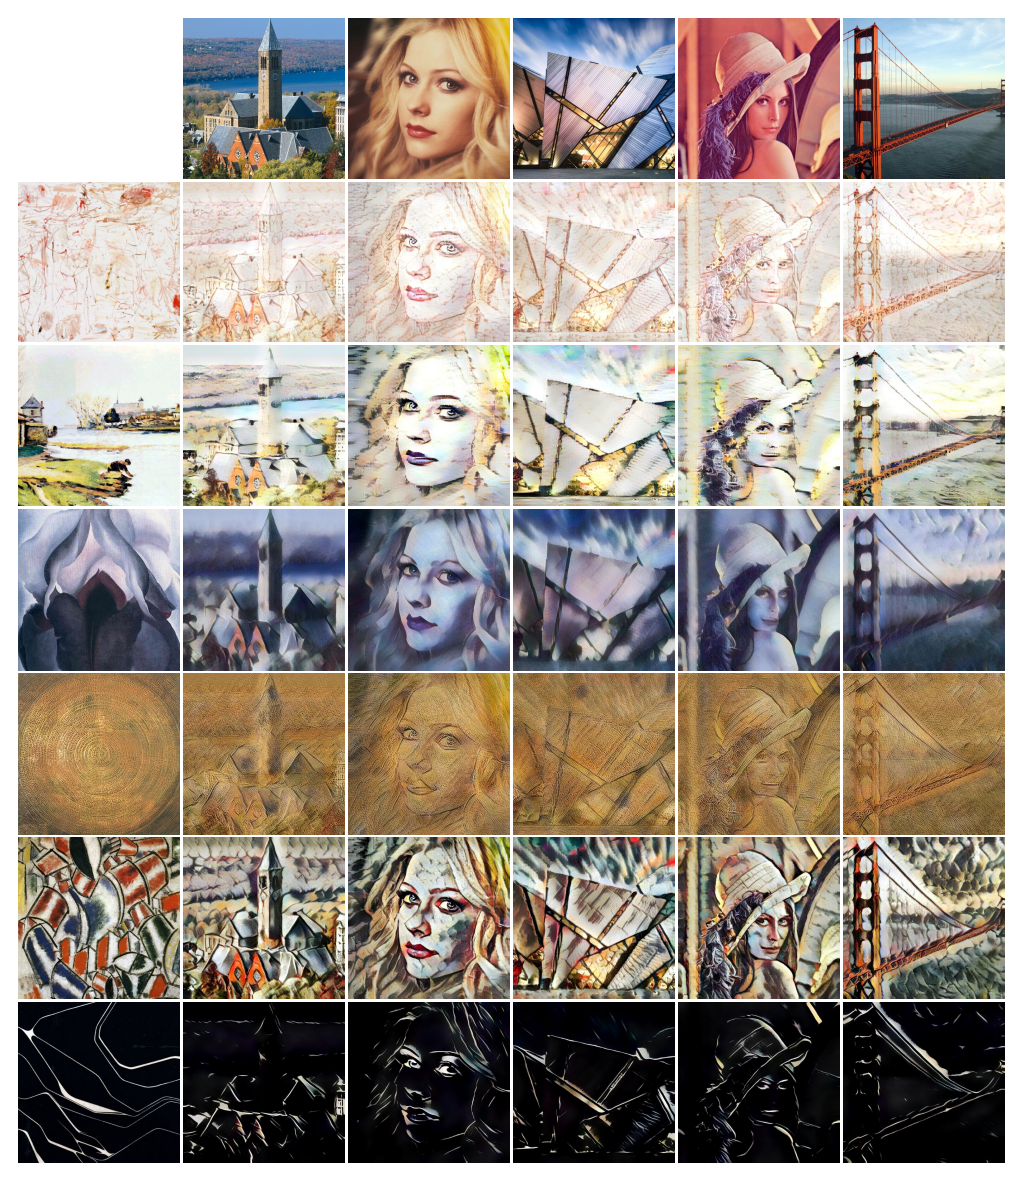
\includegraphics[width=0.7\textwidth]{images/adain_example.png}
\end{center}
  \caption{Primeri AdaIN slogovnega prenosa na slike. Vsaka vrstica si deli enak stil, vsak stolpec pa enako sliko vsebine}
  \label{AdaIN}
\end{figure}


AdaIN (ang. Adaptive Instance Normalization) \cite{huang2017adain} je normalizacijska tehnika, uporabljena za prenos poljubnega sloga med slikami v realnem času. Algoritem sestavlja kodirnik, ki sliko z vsebino in sliko sloga preslika v latentni prostor značilk in vrne značilki x in y. Sliki predstavljeni v latentnem prostoru sta nato poslani v sloj AdaIN, kateri v vsakem kanalu slik uravna srednjo vrednost $\mu$ in standardni odklon $\sigma$ značilk x slike z vsebino s srednjo vrednostjo in standardnim odklonom značilk y slike s slogom. Na koncu naučeno dekodirno omrežje generira novo slogovno spremenjeno sliko z invertiranjem izhoda AdaIN nazaj v prostor originalne slike z vsebino. 

\begin{equation}
\text{AdaIN}(x,y) = \sigma(y) \frac{x - \mu(x)}{\sigma(x)} + \mu(y),
\end{equation}

\begin{figure}[htb]
\begin{center}
  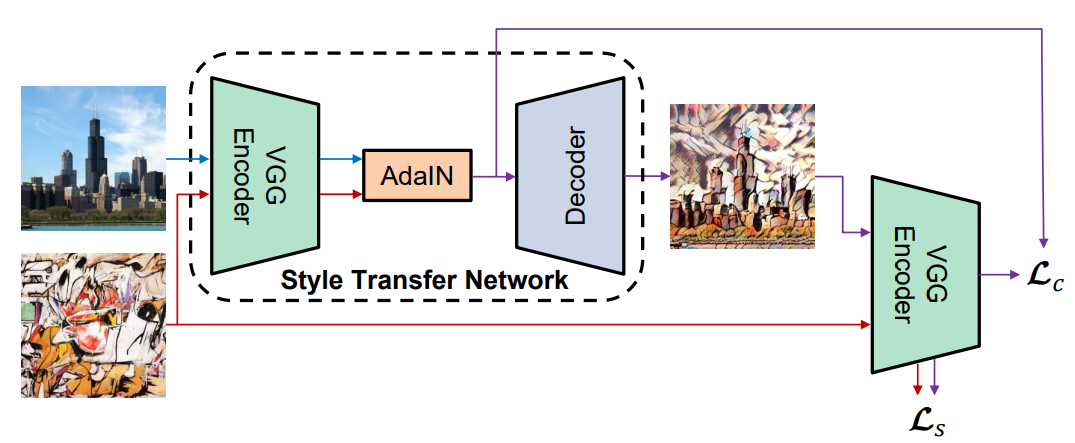
\includegraphics[width=0.7\textwidth]{images/adain_architecture.png}
\end{center}
  \caption{Arhitektura AdaIN}
  \label{AdaIN}
\end{figure}


\subsection{Arhitektura generatorja}
AdaIN je osnovna oziroma glavna sprememba dodana v novo arhitekturo StyleGAN generatorja. 
V arhitekturi StyleGAN generatorja sta na vsakem nivoju vsebovana po dva AdaIN sloja. Arhitektura generatorja pa je okoli teh slojev primerno prilagojena, kar bom opisal v tem poglavju.

Klasičen GAN generator je večplastni perceptron (ang. multilayer perceptron) oziroma nevronska mreža, pri generiranju slik je to konvolucijska nevronska mreža \cite{karras2017progressive}. Generator na vhod prejme naključni šum (ang. random noise), njegov izhod pa je generirana slika, ki je naprej podana diskriminatorju. Podobno velja za StyleGAN generator, le z določenimi dodatki in spremembami. Spremembe bom opisal v podpoglavjih Vhodni sloj, Mapirno omrežje in dodajanje sloga (ang. mapping network) ter Dodajanje šuma sinteznemu omrežju.

Generiranje slik poteka v sinteznem omrežju g, ki ga sestavlja 18 konvolucijskih slojev, ki so v 9 resolucijskih nivojih - po dve konvoluciji na enem resolucijskem nivoju. Generator omogoča povečanje dimenzije vhodne konstante iz 4x4 na 1024x1024, kar na koncu predstavlja generirano sliko. K sinteznemu omrežju so bile v okviru StyleGAN-a dodane izboljšave, ki predstavljajo nekakšno podporno infrastrukturo generatorju. 


\begin{figure}[htb]
\begin{center}
  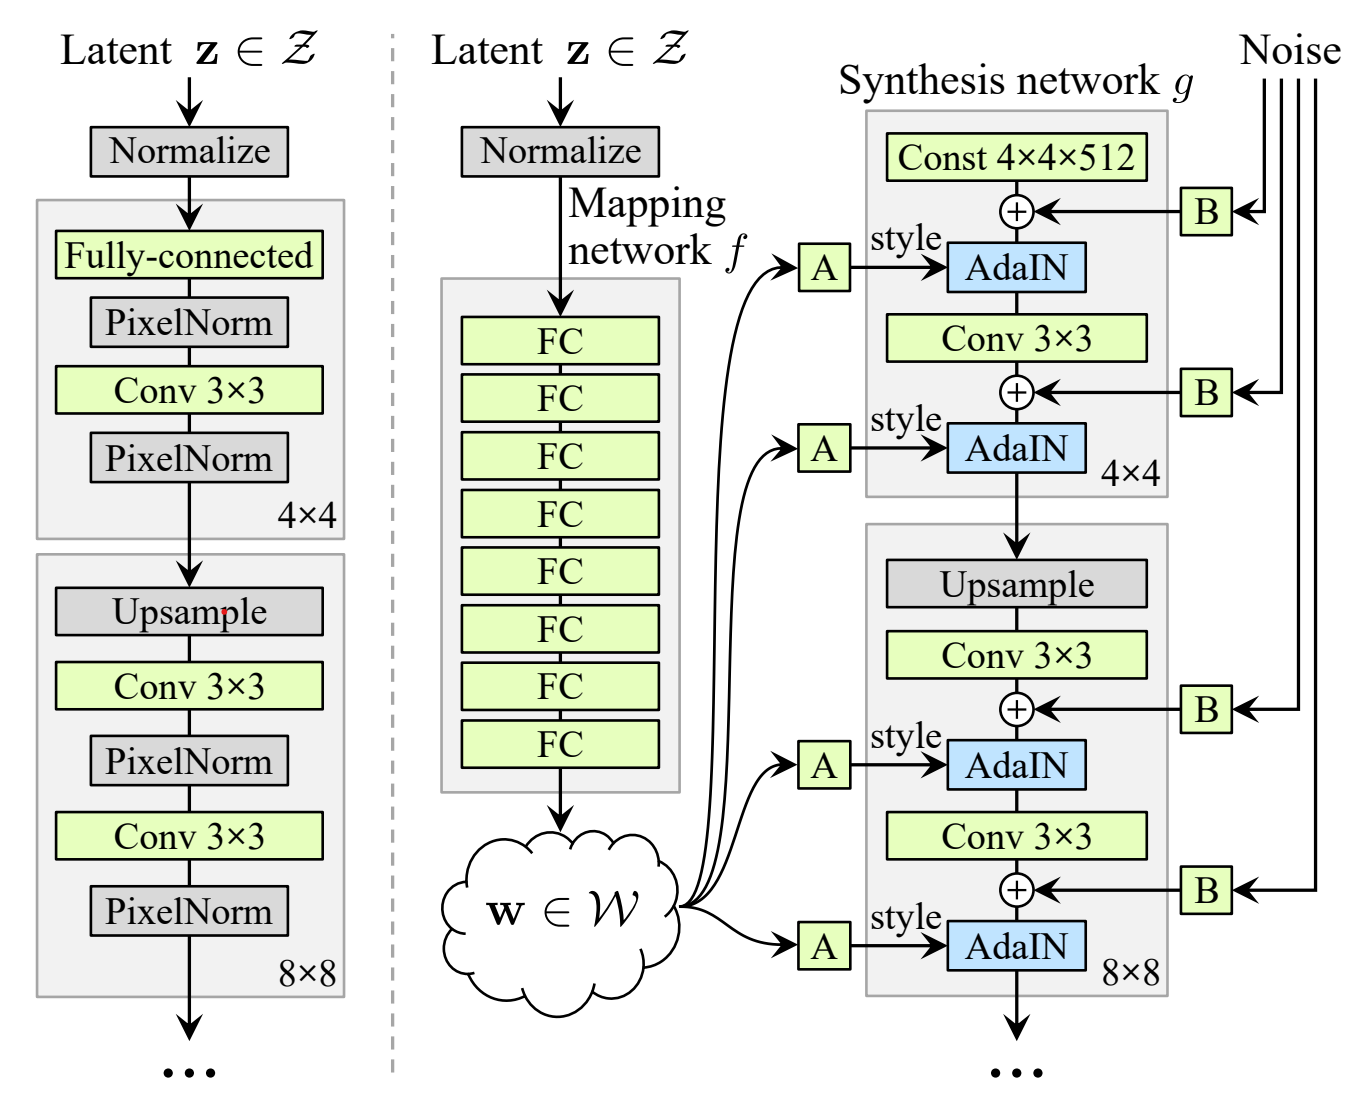
\includegraphics[width=0.7\textwidth]{images/stylegan_architecture.png}
\end{center}
  \caption{Arhitektura StyleGAN generatorja \cite{karras2019style}}
  \label{AdaIN}
\end{figure}



\subsubsection{Vhodni sloj}
StyleGAN generator se od klasičnega razlikuje že pri vhodnih podatkih. Prvi sloj pri klasičnem generatorju je tako imenovani vhodni sloj (ang. input layer), ki naključni šum na vhodu pretvori v uporabno obliko za nadalnje sloje nevronske mreže. StyleGAN pa izpusti celoten naključen vhodni sloj, namesto tega pa je vhod v NN naučena konstanta določene dimenzije 4x4x512. Konstanta na vhodnem sloju pomeni, da dejanski vhodni podatki v model pridejo le preko slogov, dodanih v AdaIN operator na vsakem sloju NN, ki so odvisni od mapirnega omrežja f.

\subsubsection{Mapirno omrežje in dodajanje sloga}

\begin{figure}[htb]
\begin{center}
  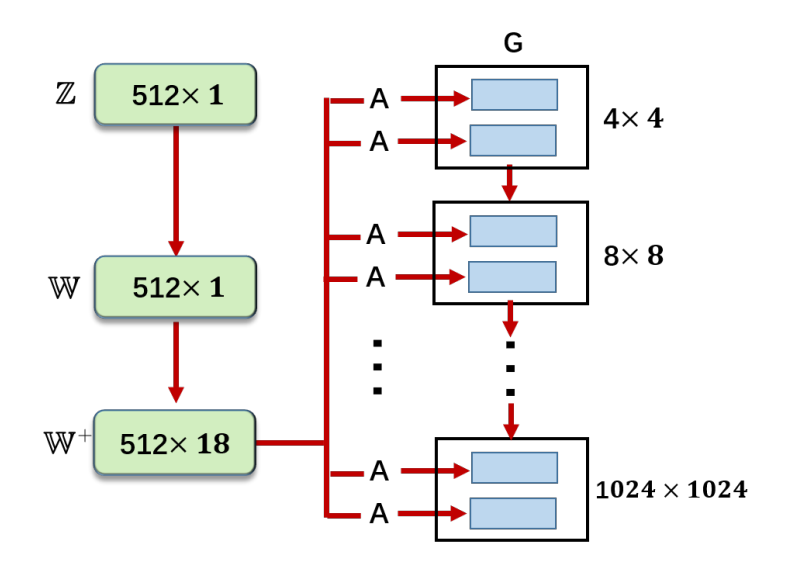
\includegraphics[width=0.7\textwidth]{images/stylegan_mapping.png}
\end{center}
  \caption{Mapirno omrežje f, ki mapira latentno kodo iz prostora Z v prostor W. W+ je razširjen prostor W. A je afina transformacija, specializirana za vsak konvolucijski sloj sinteznega omrežja g}
  \label{AdaIN}
\end{figure}

Mapirno omrežje je arhitekturno in vsebinsko po pomembnosti največja sprememba od začetnega Progressive GAN-a \cite{karras2017progressive}. V osnovi je to 8-plastni perceptron (ang. multilayer perceptron - MLP), drugače povedano nevronska mreža iz osmih popolno povezanih slojev. Na vhod dobi latentno kodo z dimenzije 512, ki pripada latentnemu prostoru Z. Naloga omrežja je mapiranje z v latentni prostor W. Izhod omrežja je latentna koda w enakih dimezij kot z - 512. Prednaučena afina transformacija A nato, za vsak izmed 18 slojev konvolucije posebej, specializira w v stile y, ki kontrolirajo AdaIN operacije po vsakem konvolucijskem slogu sinteznega omrežja g. AdaIN normalizacija deluje enako kot je bila opisana v poglavju 3.2.1, z razliko v vhodnem slogu. Vhodni slog v tem primeru ni slika sloga, vendar je to izračunan slog y na podlagi vektorja w. AdaIN operacija je torej definirana kot

\begin{equation}
\text{AdaIN}(x_{i},y) = y_{s,i} \frac{x_{i} - \mu(x_{i})}{\sigma(x_{i})} + y_{b,i},
\end{equation}

kjer je vsak feature map $x_{i}$ obravnavan posebej. Torej srednja vrednost in standardni odklon $x_{i}$ sta uravnana s srednjo vrednostjo in standardnim odklonom pripadajoče komponente sloga y.


\subsubsection{Dodajanje šuma sinteznemu omrežju}

\begin{figure}[htb]
\begin{center}
  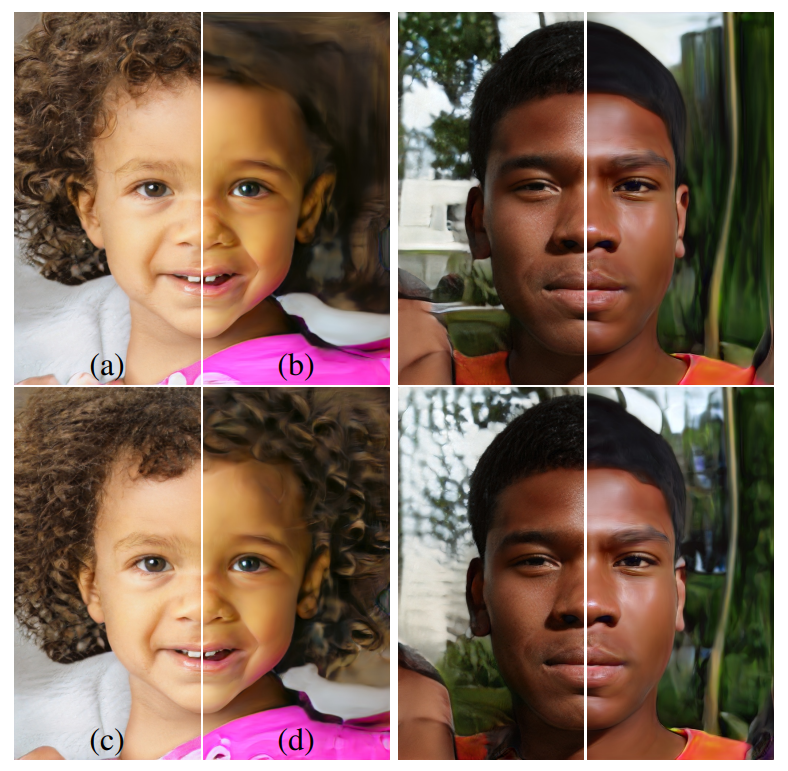
\includegraphics[width=0.5\textwidth]{images/stylegan_noise.png}
\end{center}
  \caption{(a) Šum dodan na vseh slojih. (b) Brez dodanega šuma. (c) Šum dodan v slojih podrobnosti (fine layers) ($64^2 - 1024^2$). (d) Šum dodan v slojih (coarse layers)  ($4^2 - 32^2$)}
  \label{AdaIN}
\end{figure}

Najbolj vidni aspekti stohastičnih podrobnosti v človeških portretih bi na primer bili točna postavitev las, lokacija kožnih por in peg, postavitev gub na obrazu in podobno. Za naposredno dodajanje stohastičnih podrobnosti se v model dodaja šum (ang. noise). Šum je eno kanalna slika nepovezanega Gaussovega šuma. Dodana je po vsakem konvolucijskem sloju sinteznega omrežja g. Katerkoli od aspektov podrobnosti je z dodajanjem šuma randomiziran brez, da to vpliva na celotno podobo obraza in identiteto človeka.

\begin{figure}[htb]
\begin{center}
  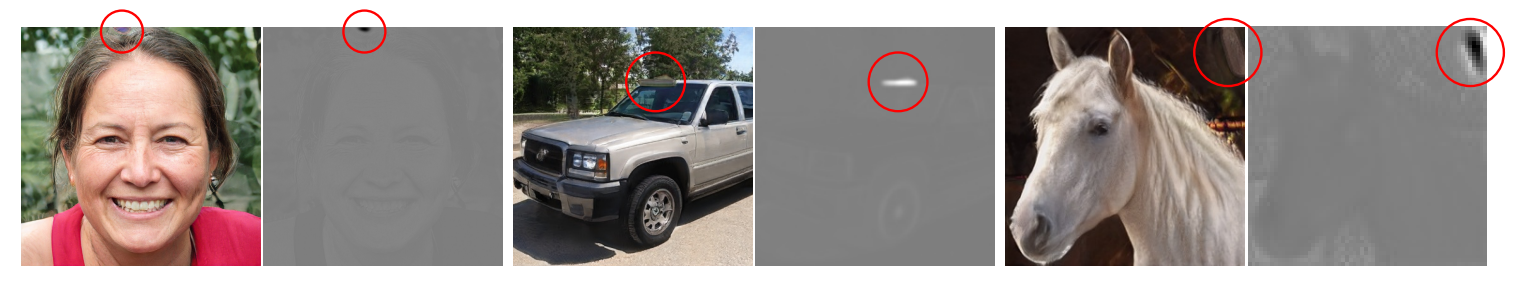
\includegraphics[width=1\textwidth]{images/stylegan_artefacts.png}
\end{center}
  \caption{Normalizacija v operaciji AdaIN StyleGAN generatorja povzroča artefakte v obliki vodnih kapelj. Niso vedno vidni na generiranih slikah, vendar jih je mogoče opaziti na aktivacijah znotraj omrežja generatorja. Problem je sistemski, saj so artefakti prisotni na vseh slikah. StyleGAN2 predlaga spremembe, ki to odpravijo. }
  \label{Artefakti}
\end{figure}



\subsection{StyleGAN2}

Kreatorji StyleGAN arhitektue so 2020 to posodobili in izdali članek \textbf{Analyzing and Improving the Image Quality of StyleGAN} \cite{Karras2019stylegan2}. V članku analizirajo več njegovih značilnih artefaktov in predlagajo spremembe v arhitekturi modela in metodah učenja modela, da bi jih odpravili. Večje spremembe so na novo oblikovana normalizacija generatorja (operacija AdaIN), ponovno preučijo postopno rast (ang. progressive growing) in regulirajo generator, in s tem spodbudijo dobro pogojenost pri preslikavi latentnih kod v slike. 

Poleg izboljšanja kakovosti slik, regulator dolžine poti (ang. Path length regularization) prinaša dodatno korist, saj je generator dosti lažje invertirati. To omogoča zanesljivo pripisovanje latentne kode poljubni sliki. Povedano drugače, iz poljubne slike lahko pridobimo latentno kodo, ki v latentnem prostoru predstavlja dober približek originalni sliki, če bi iz te latentne kode spet generirali originalno sliko. 



\subsubsection{Spremembe v arhitekturi generatorja}

\begin{figure}[htb]
\begin{center}
  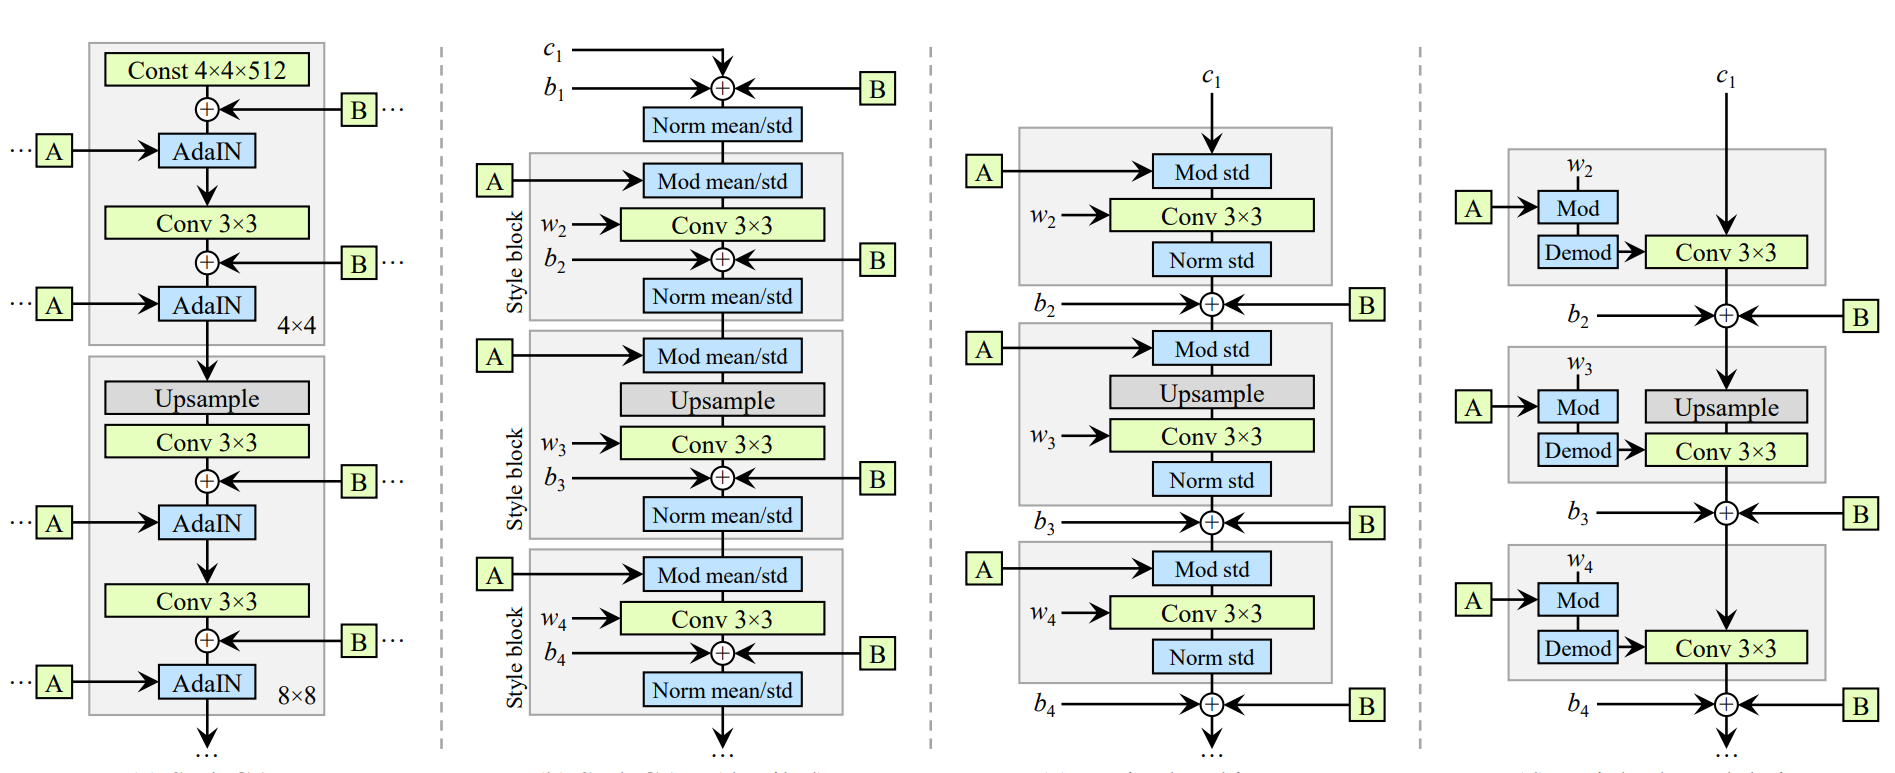
\includegraphics[width=1\textwidth]{images/stylegan2_generator.png}
\end{center}
  \caption{(a) Originalni generator StyleGAN (b) Originalni generator StyleGNA, podrobneje (c) Diagram novega StyleGAN2 generatorja (d) Operacija demodulacije}
  \label{Spremembe v arhitekturi StyleGAN2 generatorja}
\end{figure}

(a) Originalni generator StyleGAN, kjer A označuje naučeno
afino transformacijo iz W, ki ustvari slog, B pa je operacija oddajanja šuma 

(b) Isti diagram StyleGAN kot pri (a), le da prikazuje več podrobnosti. AdaIN operacija je razbita na normalizacijo in sledečo modulacijo, obe delujoči na povprečju in standardnem odklonu za vsak feature map posebej. Anotirani so tudi naučene uteži (w), pristranskosti b in konstantni vhod c ter na novo narisana siva polja, tako da je aktiven po en slog v vsakem polju. Aktivacijska funkcija (puščajoča ReLU) se vedno uporabi takoj po dodajanju pristranskosti. 

(c) Diagram novega StyleGAN2 generatorja. Odstranjene so nekatere odvečne operacije na začetku, seštevanje b (pristranskosti) in B (dodajanje šuma) sta premaknjena izven aktivnega območja sloga, kjer delujeta na normaliziranih podatkih, kar se izkaže za bolj predvidljivo (njun vpliv ni več inverzno odvisen od magnitude dodanega sloga). Pri spremenjeni arhitekturi se izkaže, da je zadostno, da modulacija in normalizacija delujeta le nad standardnim odklonom za vsak feature map - povrpečje je redundantno.

(d) Spremenjena arhitektura omogoča zamenjavo normalizacije primerov z operacijo "demodulacije", ki jo uporabimo nad utežimi w, povezane z vsako konvolucijsko plastjo. Demodulacija je operacija, ki je uporabljena namesto normalizacije primerov (AdaIN normalizacija). Deluje bolj direktno, na podlagi statistične analize o signalu, namesto dejanskih podatkih o feature mapih, vendar je zato tudi bolj šibka.


\subsubsection{Projekcija slike v latentni prostor}
Za manipulacijo poljubne slike v prostoru latentnih značilnosti je treba najprej poiskati ujemajočo latentno kodo w zanjo. Predlagatelji StyleGAN arhitekture, tega niso implementirali, bilo pa je implementirano kasneje in predstavljeno v člankih \textbf{Image2StyleGAN: How to Embed Images Into the StyleGAN Latent Space?} \cite{Image2StyleGAN2019} in \textbf{Style Generator Inversion for Image Enhancement and Animation} \cite{gabbay2019style}. Te implementacije poskušajo najti posamezno optimalno latentno kodo w za vsak sloj konvolucije, kar izboljša podobnost originalni sliki. Problem takšne implementacije pa je, da omogoča preslikavo poljubne slike, ki ne bi smela imeti reprezentacije v latentnem prostoru. 

Za nas je projekcija slike v latentni prostor najpomembnejša sprememba oziroma dodatek, ki ga predlaga StyleGAN2 arhitektura. Pridobitev latentne kode iz poljubne slike omogoča veliko lažje operacije nad slikami. Čeprav ta preslikava ni popolna, je dovolj dobra za našo uporabo.

Predlagatelji StyleGAN2 arhitekture torej implementirajo projekcijo slike v latentni prostor na tak način, da poiščejo eno latentno kodo v prvotnem, nerazširjenem latentnem prostoru, saj te ustrezajo slikam, ki bi jih lahko ustvaril generator.

Njihov implementacija se od prejšnjih razlikuje v dveh osnovnih stvareh. Prva, med optimizacijo latentni kodi dodajo zmanjšan šum, da bi čim bolj celotno preiskali latentni prostor. Druga, optimizirajo vhode stohastičnega šuma pri StyleGAN2 generatorju - jih regularizirajo, da ne prenašajo koherentnega signala ozitoma šuma. Regularizacija temelji na posodabljanju avtokorelacijskih koeficientov šuma, ki se morajo ujemati z temi Gaussovega šuma na več lestvicah.





\section{Napovedni modeli}

Cilj diplomske naloge je iz slik obrazov otrok generirati slike obrazov staršev tako, da bodo po objektivno določenih metrikah čim bolj podobni njihovim pravim staršem. V sami osnovi gre za problem napovedovanja rezultatov na podlagi pridobljenih podatkov s pomočjo prednaučenih napovednih modelov.

V prvem koraku smo uporabili StyleGAN2 projektor za pridobitev latentnih kod vseh slik, na katerih bomo izvajali učenje ter kasneje predikcijo. Slikam smo tako zmanjšali dimenzijo, tako lahko veliko lažje izvajamo računske operacije in s tem učenje napovednih modelov. Dimenzija prvotnih slik je bila 1024x1024x3, dimenzija latentne kode določene slike pa je 18x512, kar je približno 34.000-kratno zmanjšanje.

\subsection{Linearna regresija}

Linearna regresija je statistična metoda, ki se uporablja za modeliranje odvisnosti med odvisno spremenljivko in eno ali več neodvisnimi spremenljivkami. Cilj linearne regresije je najti linearno razmerje med spremenljivkami, ki se lahko uporablja za napovedovanje odvisne spremenljivke na podlagi vrednosti neodvisnih spremenljivk.



Model linearne regresije (ang. Linear Regression Model), podan z enačbo (3.4), opredeljuje odvisnost med odvisno spremenljivko $y$ in neodvisnimi spremenljivkami $x_1, x_2, ..., x_p$. Model predpostavlja, da obstaja linearno razmerje med spremenljivkami in da je vsako odstopanje od linearne zveze posledica naključne napake $\epsilon_i$. Model vključuje $p+1$ neznanih parametrov $\beta_0, \beta_1, ..., \beta_p$, ki predstavljajo odmik in naklone regresijske premice.

\begin{equation}
y_i = \beta_0 + \beta_1 x_{i1} + \beta_2 x_{i2} + \cdots + \beta_p x_{ip} + \epsilon_i
\end{equation}


Ocenjevanje z najmanjšimi kvadrati (ang. Least Squares Estimation), podano z enačbo (3.5), se uporablja za ocenjevanje vrednosti neznanih parametrov, ki minimizirajo vsoto kvadratov napak med opazovanimi vrednostmi odvisne spremenljivke in napovedanimi vrednostmi na podlagi neodvisnih spremenljivk. To se izvede z iskanjem vrednosti $\beta_0, \beta_1, ..., \beta_p$, ki minimizirajo vsoto kvadratov ostankov $\sum_{i=1}^{n} (y_i - \hat{y_i})^2$.

\begin{equation}
\hat{\beta} = \operatorname*{argmin}{\beta} \sum{i=1}^{n} \left(y_i - \beta_0 - \beta_1 x_{i1} - \beta_2 x_{i2} - \cdots - \beta_p x_{ip}\right)^2
\end{equation}

Ocenjena regresijska funkcija (ang. Estimated Regression Function), podana z enačbo (3.6), predstavlja napovedane vrednosti odvisne spremenljivke na podlagi ocenjenih vrednosti parametrov $\hat{\beta}_0, \hat{\beta}_1, ..., \hat{\beta}_p$ in vrednosti neodvisnih spremenljivk $x_1, x_2, ..., x_p$. Ostanki (ang. Residuals), podani z enačbo (3.7), predstavljajo razlike med opazovanimi vrednostmi odvisne spremenljivke in napovedanimi vrednostmi na podlagi ocenjene regresijske funkcije.

\begin{equation}
\hat{y} = \hat{\beta}_0 + \hat{\beta}_1 x_1 + \hat{\beta}_2 x_2 + \cdots + \hat{\beta}_p x_p
\end{equation}

\begin{equation}
e_i = y_i - \hat{y}_i
\end{equation}

Vsota kvadratov ostankov (ang. Sum of squared residuals), podana z enačbo (3.8), predstavlja celotno količino napake v regresijskem modelu. Celotna vsota kvadratov (ang. Total Sum of Squares), podana z enačbo (3.9), predstavlja skupno variacijo odvisne spremenljivke okoli njenega povprečja. Koeficient determinacije (ang. Coefficient of Determination) ali $R^2$ , podan z enačbo (3.10), predstavlja delež variacije odvisne spremenljivke, ki ga razloži regresijski model. Vrednost $R^2$, ki je blizu 1, kaže na dobro prileganje med modelom in podatki.


\begin{equation}
SSE = \sum_{i=1}^{n} e_i^2
\end{equation}

\begin{equation}
SST = \sum_{i=1}^{n} \left(y_i - \bar{y}\right)^2
\end{equation}

\begin{equation}
R^2 = \frac{SST - SSE}{SST} = 1 - \frac{SSE}{SST}
\end{equation}


Standardna napaka ocene (ang. Standard Error of the Estimate), podana z enačbo (3.11), je mera povprečne razdalje med opazovanimi vrednostmi odvisne spremenljivke in napovedanimi vrednostmi na podlagi regresijskega modela. Interval zaupanja (ang. Confidence Interval) za $\beta_j$ , podan z enačbo (3.12), predstavlja območje vrednosti, v katerem je verjetno, da bo prava vrednost $\beta_j$, s določeno stopnjo zaupanja.

\begin{equation}
s = \sqrt{\frac{SSE}{n - p - 1}}
\end{equation}

\begin{equation}
\hat{\beta}j \pm t{\alpha/2,n-p-1} \frac{s}{\sqrt{\sum_{i=1}^{n} \left(x_{ij} - \bar{x}_j\right)^2}}
\end{equation}

kjer je $t_{\alpha/2,n-p-1}$ percentil $1-\alpha/2$ porazdelitve $t$ z $n-p-1$ stopnjami prostosti.


Na splošno funkcije, ki opisujejo linearne regresije, delujejo skupaj za oceno parametrov linearnega odnosa med odvisno spremenljivko in eno ali več neodvisnimi spremenljivkami ter ocenjevanje prileganja regresijskega modela podatkom. Model se lahko uporablja za napovedovanje vrednosti odvisne spremenljivke na podlagi vrednosti neodvisnih spremenljivk, ocenjene parametre pa je mogoče interpretirati za razumevanje narave odnosa med spremenljivkami. 


\subsubsection{Matrična oblika}
Vse enačbe, ki opisujejo linearno regresijo, v matrični obliki. Ta je bolj relevantna za nadaljevanje, saj se bolj enostavno odraža v kodi.

The hypothesis function:

$h_{\boldsymbol{\beta}}(\mathbf{X}) = \mathbf{X}\boldsymbol{\beta}$

The loss function:

$J(\boldsymbol{\beta}) = \frac{1}{2n} (\mathbf{X}\boldsymbol{\beta} - \mathbf{y})^T(\mathbf{X}\boldsymbol{\beta} - \mathbf{y})$

The gradient of the loss function:

$\nabla_{\boldsymbol{\beta}} J(\boldsymbol{\beta}) = \frac{1}{n} \mathbf{X}^T(\mathbf{X}\boldsymbol{\beta} - \mathbf{y})$

The normal equation:

$\boldsymbol{\beta} = (\mathbf{X}^T\mathbf{X})^{-1}\mathbf{X}^T\mathbf{y}$

The prediction:

$\hat{\mathbf{y}} = \mathbf{X}\boldsymbol{\beta}$

The sum of squared residuals:

$SS_{res} = (\mathbf{y} - \hat{\mathbf{y}})^T(\mathbf{y} - \hat{\mathbf{y}})$

The total sum of squares:

$SS_{tot} = (\mathbf{y} - \bar{\mathbf{y}})^T(\mathbf{y} - \bar{\mathbf{y}})$

The coefficient of determination:

$R^2 = 1 - \frac{SS_{res}}{SS_{tot}}$

The standard error of the estimate:

$SE(\boldsymbol{\epsilon}) = \sqrt{\frac{1}{n-p-1} SS_{res}}$

The confidence interval for $\beta_j$:

$CI(\beta_j) = \beta_j \pm t_{\alpha/2,n-p-1}SE(\hat{\beta_j})$

where $t_{\alpha/2,n-p-1}$ is the $1 - \alpha/2$ percentile of the $t$-distribution with $n-p-1$ degrees of freedom.



\subsection{Ridge normalizacija}

Ridge normalizacija, znana tudi kot L2 regularizacija, je tehnika, ki se uporablja za preprečevanje preprileganja v modelih linearne regresije s dodajanjem kazenskega člena v funkcijo izgube. Ta kazenski člen je sorazmeren s kvadratom magnitude koeficientov linearne regresijskega modela. S tem kazenskim členom je model spodbujen k manjšim vrednostim koeficientov, kar zmanjša kompleksnost modela in preprečuje preprileganje.

Matematično se funkcija izgube Ridge regresije lahko zapiše kot:

\begin{equation*}
L(\mathbf{y}, \mathbf{X}, \boldsymbol{\beta}) = (\mathbf{y} - \mathbf{X} \boldsymbol{\beta})^T (\mathbf{y} - \mathbf{X} \boldsymbol{\beta}) + \lambda \boldsymbol{\beta}^T \boldsymbol{\beta}
\end{equation*}

kjer je $\mathbf{y}$ vektor vrednosti ciljne spremenljivke, $\mathbf{X}$ matrika vrednosti napovednih spremenljivk, $\boldsymbol{\beta}$ vektor koeficientov, ki jih je treba oceniti, $n$ število opazovanj, $\lambda$ pa je hiperparameter, ki nadzoruje jakost kazenskega člena.

Prvi člen v funkciji izgube predstavlja povprečno kvadratno napako med predvidenimi vrednostmi in dejanskimi ciljnimi vrednostmi, drugi člen pa je L2 kazenski člen, ki krči ocene koeficientov proti nič. Hiperparameter $\lambda$ nadzira ravnovesje med tema dvema členoma in večje vrednosti $\lambda$ vodijo v manjše ocene koeficientov.

Ocene koeficientov Ridge regresije se lahko pridobijo s pomočjo naslednje enačbe:

\begin{equation*}
\boldsymbol{\beta} = (\mathbf{X}^T \mathbf{X} + \lambda \mathbf{I})^{-1} \mathbf{X}^T \mathbf{y}
\end{equation*}


kjer je $\mathbf{I}$ identitetna matrika. Ta enačba je podobna enačbi za običajni najmanjši kvadrat, vendar s dodatkom člena $\lambda$.

Ridge regresija na splošno dodaja regularizacijski člen v model linearne regresije, kar pomaga zmanjšati preprileganje in izboljšati splošno učinkovitost modela.





\subsubsection{Izbira značilk za linearno regresijo}
V našem primeru je neodvisna spremenljivka latentna koda, pridobljeno iz določenega obraza otroka. Model pa napove odvisno spremenljivko, katere polovica predstavlja latentno kodo obraza mame, polovica pa latentno kodo obraza očeta. Značilke lahko sestavimo na več različnih načinov, najboljšega pa lahko določimo s poskušanjem. Dve možnosti, ki nam takoj prideta na misel sta zaporedno sestavljena značilka iz latentnih kod mame in očeta in izmenično sestavljena značilka iz latentnih kod mame in očeta. To je kasneje bolj podrobno opisano v poglavju \textbf{4.4 Lastna implementacija}



\chapter{Implementacija lastne metode}
\section{Struktura projekta}
Projekt je narejen v okviru sistema za upravljanje paketov Conda \cite{conda}, tako je lahko pognan s pomočjo Conde na katerem koli računalniku neodvisno od že nameščenih Python knjižnic. Conda omogoča enostavno vzpostavitev Python virtualnega okolja, znotraj katerega na začetku namestimo vse potrebne knjižnice, kodo pa potem poganjamo na Python prevajalniku iz Conda virtualnega okolja.

Pri razvoju smo uporabljali sistem za nadzor različic (ang. Version control system) GitHub \cite{github}, ki je predvsem omogočil enostavnejšo integracijo dveh zunanjih modulov StyleGAN2 (v repozitoriju NVlabs/stylegan2-ada-pytorch) \cite{stylegan2adapytorch} in InterfaceGAN (v repozitoriju genforce/interfacegan) \cite{interfacegan} v projekt. S pomočjo GitHubovih submoddulov smo v projekt vključili obe zbirki podatkov NOKDB in PPLDB, za katera smo ustvarili ločena repozitorija za bolj efektivno razmnoževanje projekta v prihodnosti.

\subsection{Organizacija kode}

Celoten projekt zajema več repozitorijev. 




\subsection{Struktura nabora slikovnih podatkov}
\subsubsection{NOKDB \cite{}}
Za učenje napovednih modelov potrebujemo čim bolj kvalitetne podatke, saj je od njih precej odvisna kakovost naučenih modelov. Zato smo uporabili nov nabor podatkov, ki omogoča učenje modelov na podlagi sorodstev. Next Of Kin (NOK) vsebuje 3690 512×512 slik visoke ločljivosti obrazov 553 različnih ljudi z veliko etnično in starostno raznolikostjo. V nabor podatkov so vključeni tudi metapodatki o sorodstvenih vezeh, starosti, etnični pripadnosti, spolu in izrazu obraza.

Nabor podatkov vsebuje več kot 120.000 trojic oče - mama - otrok na katerih je potekalo učenje modelov. Vse slike v naboru podatkov so bile predprocesirane. Najprej so bili poiskani obrazni atributi in glede na njihovo pozicijo so bile slike obrezane in pravilno orientirane. Nato so bile vse slike projecirane v W+ latentni prostor (latentni prostor prednaučenega StyleGAN2 FFHQ modela), latentna koda (iid.npz) se nahaja poleg vsake izmed slik. Na koncu so bili dodani metapodatki o spolu, etnični pripadnosti vsaki osebi in starost in podatek o izrazu na obrazu vsaki izmen slik.

Podani so tudi uradni učni, validacijski in testni split, kjer so trojice oče - mama - otrok razporejene tako, da se slike specifičnega otroka ne pojavijo v več kot enem izmed njih. Spliti so definirani v datotekah nokdb-samples, poleg treh ki se uporabljajo za učenje in izboljševanje modela smo pripravili še dva druga splita, ki se uporabljata za generiranje realnih slik staršev iz slik otrok ali sli otrok iz lik staršev. Latentne kode za te slike pridejo v NOKDB iz slikovne podatkovne zbirke PPLDB.

\begin{center}
  \begin{tabular}{|l|l|}
  \hline
  Značilnosti nabora podatkov & Število \\
  \hline
  persons & 1116 \\
  images & 3690 \\
  images per person & 3.31 \\
  image sample combinations & 127,719 \\
  father/mother/son person triplets & 116 \\
  father/mother/daughter person triplets & 133 \\
  image resolution & 512x512 \\
  \hline
  \end{tabular}
\end{center}

\begin{center}
  \begin{tabular}{|l|l|}
  \hline
  Pot & Opis \\
  \hline
  |- nokdb-images.csv & Seznam slik z atributi \\
  |- nokdb-persons.csv & Seznam oseb z atributi \\
  |- nokdb-samples-test.csv & Trojčki oče-mama-otrok (testni) \\
  |- nokdb-samples-train.csv & Trojčki oče-mama-otrok (učni) \\
  |- nokdb-samples-validation.csv & Trojčki oče-mama-otrok (validacijski) \\
  |- nokdb-samples-all.csv & Trojčki oče-mama-otrok (vsi) \\
  |- nokdb-samples-real-c2p.csv & Trojčki oče-mama-otrok za generiranje staršev \\
  |- nokdb-samples-real-p2c.csv & Trojčki oče-mama-otrok za generiranje otrok \\
  |- nokdb-normalization.npz & W vektor normalizacija povprečje \\ & in standardni odklon za vsako dimenzijo \\
  \hline
  \end{tabular}
\end{center}

\begin{center}
  \begin{tabular}{|l|l|}
  \hline
  Poti & Opis \\
  \hline
  |- pid0/ & Direktorij, ki vsebuje nabor podatkov osebe `pid0` \\
  |----- iid0.png & Slika `iid0`, ki pripada osebi `pid0` \\
  |----- iid0.npz & StyleGAN2 latentna koda slike `iid0` \\
  |----- iid1.png & Slika `iid1`, ki pripada osebi `pid0`\\
  |----- iid1.npz & StyleGAN2 latentna koda slike `iid1`\\
  |- pid1/ & \\
  |----- ... & \\
  |- ... & \\
  \hline
  \end{tabular}
\end{center}


\subsubsection{PPLDB}
Medtem ko je NOKDB usmerjen pretežno v učenje modelov in kvalitete teh, smo opazili potrebo po lastnem naboru podatkov, v katerem bodo hranjeni slikovni podatki iz spletne aplikacije, kjer je model uporabljen. Tu se predvsem kopičijo slike, ki so lahko kasneje ali avtomatsko migrirane v NOKDB, za ponovno učenje napovednih modelov. Podobno kot NOKDB tudi PPLDB na začetku slike predprocesira. Najprej so slike obrezane in rotirane na podlagi zaznanih obraznih atributov. Nato so projecirane v StyleGAN2 FFHQ latentni prostor W+, latentne kode pa so shranjene, poleg podatkov o loss in gain pri projekciji, v PPLDB.  

V datoteki nokdb-mapping.csv so hranjeni podatki o mapiranju oseb iz PPLDB v NOKDB. Zapisano je njihov pid iz PPLDB in njihov pid iz NOKDB. V datoteki couples.csv so hranjeni podatki o parih oseb, katerim lahko generiramo otroka. Potrebna je predhodna migracija podatkov o paru iz PPLDB v NOKDB.

\begin{center}
  \begin{tabular}{|l|l|}
  \hline
  Pot & Opis \\
  \hline
  |- couples.csv & Seznam parov, katerim generiramo otroka \\
  |- nokdb-mapping.csv & Seznam oseb z pripisanim NOKDB pid \\
  \hline
  \end{tabular}
\end{center}

\begin{center}
  \begin{tabular}{|l|l|}
  \hline
  Poti & Opis \\
  \hline
  |- pid0/ & Direktorij, ki vsebuje podatke osebe `pid0` \\
  |---- latents/ & Direktorij, ki vsebuje latentne podatke osebe `pid0` \\
  |-------- latents\_pid0\_iid0/ & Direktorij, ki vsebuje latentne podatke slike `pid0\_iid0` \\
  |------------ target.png & Predprocesirana slika `iid0`, ki pripada osebi `pid0` \\
  |------------ proj.png & Slika, pripadajoča generirani latentni kodi \\
  |------------ projected\_w.npz & Generirana latentna koda v prostoru W+ \\
  |------------ loss.png & Graf loss in dist, glede na korak projekcije \\
  |-------- latents\_pid0\_iid1/ & Direktorij, ki vsebuje latentne podatke slike `pid0\_iid0` \\
  |------------ iid1.png & Predprocesirana slika `iid1`, ki pripada osebi `pid0`\\
  |------------ iid0.png & Predprocesirana slika `iid0`, ki pripada osebi `pid0` \\
  |---- aligned/ & Direktorij, ki vsebuje predprocesirane osebe `pid0` \\
  |-------- pid0\_iid0.png & Predprocesirana slika `iid0`, ki pripada osebi `pid0` \\
  |-------- pid0\_iid1.png & Predprocesirana slika `iid1`, ki pripada osebi `pid0`\\
  |---- pid0\_iid0.png & Originalna slika `iid0`, ki pripada osebi `pid0`\\
  |---- pid0\_iid1.png & Originalna slika `iid1`, ki pripada osebi `pid0`\\
  |- pid1/ & Direktorij, ki vsebuje podatke osebe `pid1`\\
  |----- ... & \\
  |- ... & \\
  \hline
  \end{tabular}
\end{center}



  
\section{Opis uporabljenih tehnologij in metod}
\subsection{StyleGAN}
\subsection{Interfacegan}
\subsection{Wandb}

\section{Skupna implementacija}
Matjaž Mav je pripravil osnovno implementacijo, katero sem v okviru moje diplomske naloge samo razširil in v določenih delih spremenil ter dopolnil. Matjaž je najprej implementiral vmesnik za pridobivanje strukturiranih podatkov iz slikovne podatkovne zbirke NOKDB na več različnih načinov - datoteke v direktoriju fri-2022-diploma/src/dataset. V direktoriju fri-2022-diploma/src/utils je implementiral podporne mehanizme za izvajanje programa - vmesnik za StyleGAN2 submodul, funkcije za vizualizacijo in funkcije za pridobivanje podatkov iz GitHuba (prenos zbirke podatkov). V direktoriels so delno dokočane implementacije različnih napovednih modelov, ki jih je Matjaž testiral.

\subsection{Vmesnik za pridobivanje strukturiranih podatkov iz slikovne podatkovne zbirke NOKDB}
Osnovna naloga vmesnika je pridobivanje podatkov - latentnih kod, iz zbirke slikovnih podatkov NOKDB, s katerimi potem operiramo pri učenju, validaciji ali testiranju modelov. Uporabljen je tudi za pridobivanje latentnih kod, ki se uporabijo za generiranje slik staršev oziroma otrok iz realnih slik. 




\begin{figure}[htb]
\begin{center}
  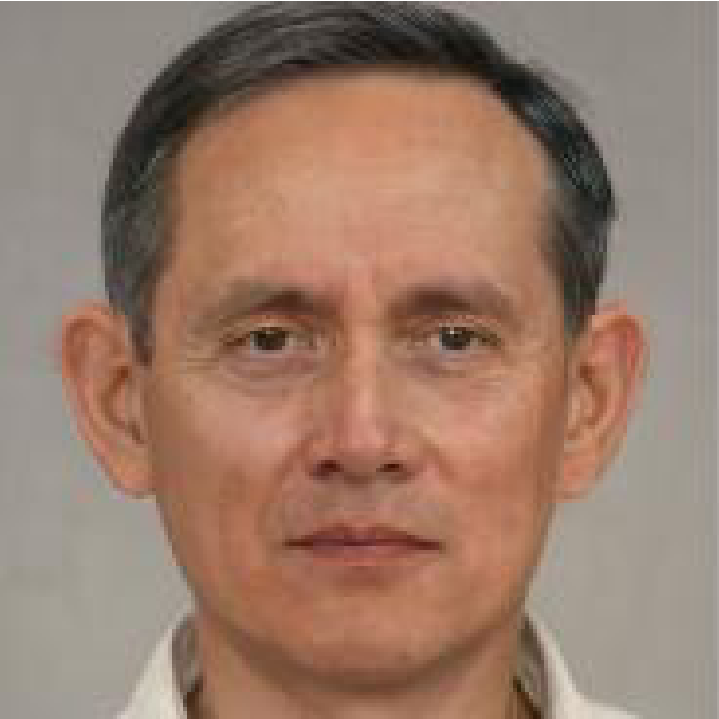
\includegraphics[width=0.7\textwidth]{images/mean_before.png}
\end{center}
  \caption{Slike, ki predstavljajo eno osebo v zbirki podatkov NOKDB}
  \label{Slike, ki predstavljajo eno osebo v zbirki podatkov NOKDB}
\end{figure}


\begin{figure}[htb]
\begin{center}
  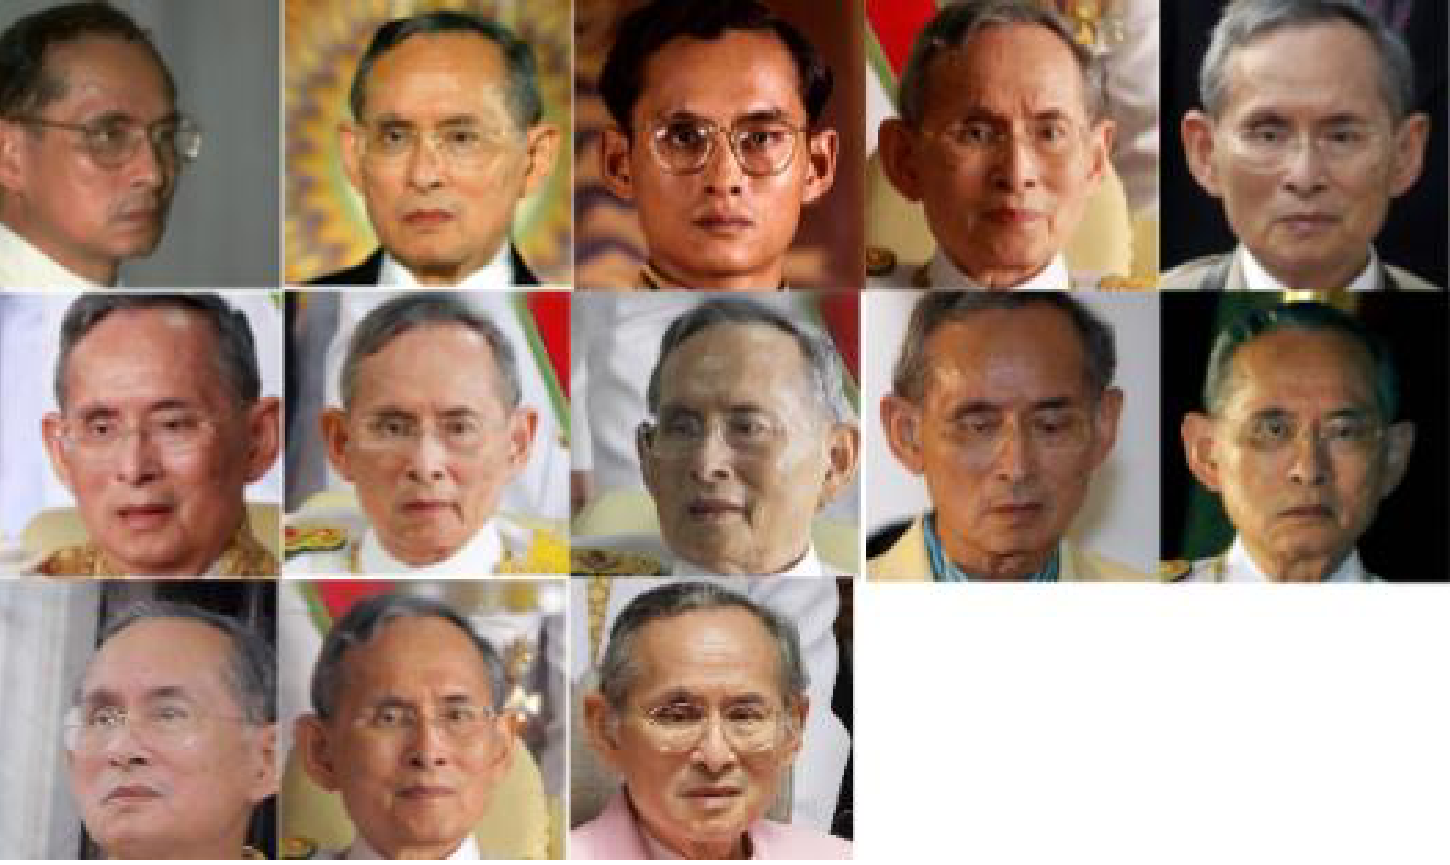
\includegraphics[width=0.5\textwidth]{images/mean_after.png}
\end{center}
  \caption{Povprečna slika osebe, generirana iz povprečne latentne kode vseh slik te osebe v zbirki podatkov NOKDB}
  \label{Povprečna slika osebe, generirana iz povprečne latentne kode vseh slik te osebe v zbirki podatkov NOKDB}
\end{figure}

Vmesnik je implementiran kot Python razred, kateremu ob inicializaciji podamo določene parametre, od katerih je odvisno kateri podatki se pridobijo iz podatkovne zbirke NOKDB. Osnovna funkcija razreda je dovajanje podatkov (latentnih vektorjev) v razredno spremenljivko data, odvisno od podanega splita - train/validation/test oziroma P2C ali C2P. Informacije o tem kateri latentni vektorji (katera starša pripadata kateremu otroku in obratno) se naložijo v spremenljivko data pa vmesnik pridobi iz datotek nokdb-samples, odvisno od podanega splita.
 
Funkcija, v kateri je implementirano nalaganje vektorjev je zasnovana tako, da latentne kode posameznega človeka združi v eno - naredi povprečje vseh latentnih kod, ki se potem uporabi v nadaljnem napovedovanju (učenje/validacija/testiranje oziroma generiranje rezultatov). Takšen način se je izkazal za najbolj učinkovitega pri končnem generiranju rezultatov. Poleg opisanega vmesnika, ki pridobi s povprečjem združeno latentno kodo posameznika, smo implementirali tudi druge, vendar se niso izkazali za tako natančne pri nadaljnem napovedovanju.  




\subsection{Vmesnik za StyleGAN2 submodul}
Uporaba StyleGAN2 arhitekture, je omogočena skozi vmesnik implementiran v datoteki fri-2022-diploma/src/utils/stylegan.py. V okviru vmesnika sta za uporabo podani dve osnovni StyleGAN2 operaciji project in generate, z različnimi možnostmi podajanja argumentov. Vmesnik izvaja python skripte definirane v submodulu repozitorija stylegan2-ada-pytorch \cite{stylegan2adapytorch} preko Docker zabojnika nad sliko stylegan2-ada-pytorch:latest, tako je zasnovan robustno, saj ni neposredno odvisen od okolja, v katerem ga poganjamo.

\subsection{Napovedni modeli}
Matjaž Mav je v okviru svoje naloge implementiral in testiral več napovednih modelov, vendar so bili ti narejeni za generacijo sli otrok na podlagi slik staršev, jaz pa v svoji nalogi potrebujem napovedni model za napovedovanje staršev iz otrok. 

\section{Lastna implementacija}
Osnovno implementacijo sem sam razširil predvsem z novim modelom, ki iz slik otrok generira slike staršev, za kar sem moral prilagoditi tudi ostale podporne mehanizme. 
Drugi dodatek pa je implementacija in integracija nove podatkovne zbirke PPLDB, ki omogoča vnos novih oseb in razmerij med osebami v podatkovno zbirko NOKDB. Zadnja stvar, ki sem jo naredil je ovrednotenje generiranih slik in vizualizacija teh rezultatov.

\subsection{PPLDB}
Za implementacijo nove zbirke podatkov in njenih podpornih mehanizmov smo se odločili zaradi potrebe po širši uporabi sistema. PPLDB omogoča dodajanje novih oseb in njenih slik v celoten sistem. V nadaljevanju bomo glede na tok podatkov ene osebe opisali funkcionalnosti sistema PPLDB.

Slike osebe shranimo v nov direktorij poimenovan po osebi v direktoriju 
fri-2022-diploma/src/dataset/ppldb, npr. \break
fri-2022-diploma/src/dataset/ppldb/vid/slika1.jpg,
Ob naslednjem zagonu programa se sproži podatkovni cevovod, ki bo omogočil generiranje slik staršev. Najprej se požene funkcija, ki dodani osebi pripiše identifikacijsko številko PPLDB in slike prestavi v nov direktorij, ter jih hkrati preimenuje v standardizirano ime "ime\_iid"npr. \break
fri-2022-diploma/src/dataset/ppldb/people/ppldb\_pid/vid\_1.jpg. 
Takoj za tem poteče predprocesiranje slik, kjer so obrezane in rotirane na podlagi zaznanih obraznih atributov. To je ključnega pomena za nadaljno uporabo slik pri generiranju latentnih kod, kar je naslednji korak. Vsaka slika, ki je bila uspešno predprocesirana je nato projecirana v latentni prostor s pomočjo StyleGAN2 funkcije project, ki jo kličemo preko vmesnika za StyleGAN2 submodul. Rezultat projekcije so latentne kode, graf spreminjanja rezultata funkcije izgube in razdalje skozi iteracije projekcije in slika, ki prikazuje generirano latentno kodo v originalnem nelatentnem prostoru.

Osnovna funkcija zbirke podatkov PPLDB je le shranjevanje latentnih kod, ki pripadajo realnim slikam. Njena uporabnost pa je v tem, da dovaja podatke v zbirko podatkov NOKDB preko katere kasneje poteka pridobivanje podatkov za generiranje slik staršev.

\subsection{Generacija slik staršev}
Celoten proces generacije slik staršev s pomočjo že naučenega modela je razdeljen na več manj obsežnih operacij. Najprej, poteče operacija opisana v prejšnjem podpoglavju - populacija PPLDB baze s latentnimi kodami slik in migracija teh latentnih kod in ostalih podatkov v podatkovno zbirko NOKDB. 

Nato se preko vmesnika, opisanega v poglavju \textbf{Vmesnik za pridobivanje strukturiranih podatkov iz slikovne podatkovne zbirke NOKDB} pridobijo podatki, ki jih nato pošljemo v določen model. Podatki so povprečne latentne kode, izračunane iz latentnih kod vseh slik določene osebe.

Prednaučen model linearne regresije potem generira latentne kode najbolj verjetnih staršev za podane latentne kode. 

Zadnji korak pred ovrednotenjem rezultatov je generacija slik iz generiranih latentnih kod. Končne slike generiramo s pomočjo modula opisanega v poglavju \textbf{Vmesnik za StyleGAN2 submodul}. Znotraj modula kličemo StyleGAN2 funkcijo generate, ki podanemu nizu latentnih kod generira pripadajoče slike. Preden poteče ovrednotenje rezultatov slike še zložimo v kolaž, da je pregledovanje rezultatov bolj pregledno.



\subsection{Rezultati}

Predstavili bomo rezultate pridobljene na dva različna načina, glede na vhodne podatke. 
Prvi način so rezultati pridobljeni le s pomočjo podatkovne zbirke NODKB, kjer je model naučen in testiran le na podatkih iz te zbirke (ločeni podatki za učenje in testiranje modela).
Pri drugem načinu pa bomo predstavili rezultate pridobljene s pomočjo modela naučenega na vseh NOKDB podatkih, testiranje pa poteka na lastnih oziroma zunanjih slikah, ki smo jih v NOKDB podatkovni zbirko vnesli preko sistema PPLDB.
V poglavju Ovrednotenje bomo rezultate kvalitativno ovrednotili s pomočjo tehnik razpoznavanja obrazov, v tem poglavju pa bomo le podali slikovne rezultate in jih vizualno opisali ter razložili možne napake v generiranju oziroma opredelili vizualne artefakte.


\subsubsection{NOKDB rezultati}
Ti rezultati so bili pridobljeni z enakim načinom kot poteka ovrednotenje, opisano kanseje. V tem poglavju bom le vizualno predstavil pridobljene slike.
Na prvi pogled delujejo generalno rezultati precej dobri, brez veliko vidnih artefaktov, vendar se tudi ti občasno pojavljajo. Artefakti se po navadi pojavijo v primerih, kjer poskušamo generirati starše odraslemu človeku. Razlog za to je v tem, da modela nismo učili na slikah, kjer bi bili otroci že starejši (ali pa je bilo teh primerov v učni množici premalo). 
Temu bi se lahko izognili, če bi ob generiranju preverjali starost otroka in ustrezno prilagodili sliko (oziroma latentno kodo) tako, da bi mu zmanjšali starost brez spremembe identitete. To bi lahko impelementirali s pomočjo submodula InterfaceGAN. 

Če vizualno primerjamo generirane starše realnim, ugotovimo da model bolje napoveduje mamo kot očeta, česar nismo mogli spremeniti kljub drugačni postavitvi značilk pri vhodu v linearno regresijo. Za ugotovitev zakaj je to tako, bi potrebovali več časa.

\subsubsection{Lastni rezultati}


\chapter{Ovrednotenje rezultatov}

Da bi ovrednotili podobnost identitet generiranih slik staršev z realnimi slikami bomo uporabili različne modele za razpoznavo obrazov.
Takšnih modelov je kar nekaj, mi bomo uporabljali tri precej splošno razširjene FaceNet \cite{facenet}, ArcFace \cite{arcface} in VGG-Face \cite{vggface}.


\section{Deepface knjižnica za razpoznavo obrazov}
Deepface je python knjižnica oziroma ogrodje, ki omogoča hitro in enostavno uporabo state-of-the-art modelov za razpoznavo obrazov, prepoznavo obrazov, podobnost obrazov in analizo obraznih atributov. 
Vsebuje implementacije VGG-Face, Facenet, Facenet512, OpenFace, DeepFace, DeepID, ArcFace, Dlib in SFace modelov.
Uporabili smo jo, ker je zelo enostavna za uporabo in smo jo zlahka vključili v lastno implementacijo razreda, namenjenega ovrednotenju rezultatov.
Knjižico smo uporabili le za eno funkcijo, ki iz določene slike obraza pridobi skrčeno predstavitev oziroma nek vektor, ki predstavlja atribute obraza (ang. embedding).

\section{Ovrednotenje}
Po uporabi Deepface knjižnice za pridobitev skrčene predstavitve obraza generirane slike in obraza prave slike enakega primera, ju primerjamo s pomočjo neke razdalje. 
Razdalja uporabljena v implementaciji je kosinusna, saj je najbolj primerna za vektorje takšnih dimenzij. 
Pri ovrednotenju smo izbrali strategijo pozitivnih parov, za razliko od drugih podobnih implementacij, ki uporabljajo strategijo pozitivnih in negativnih parov. To pomeni, da smo primerjali le realno sliko starša z generirano sliko starša (strategija pozitivnih parov). 
Nismo pa tudi primerjali razlike realne slike starša s naključno generirano sliko starša (strategija negativnih parov), saj menimo, da ta razlika ni tako pomembna kot podobnost pozitivnega para.




Napovedni model smo v primeru generiranja slik obrazov staršev, na podlagi slik obrazov otrok, ovrednotili tako, da smo primerjali realne slike obrazov staršev z generiranimi slikami obrazov staršev. 
To smo za vsak primer naredili s tremi modeli prepoznave obrazov ArcFace, Facenet in VGG-Face. 

Da smo dobili čim bolj spodobne rezultate smo ovrednotenje opravili večkrat, po podobnem principu kot poteka prečna validacija modela (ang. cross validation). To pomeni, da smo model vrednotili v več iteracijah in na koncu vzyeli povprečje rezultatov vseh iteracij, tako so rezultati bolj reprezentativni, kot če bi opravili le eno iteracijo ovrednotenja. Najprej smo razdelili vse otroke na $k$ množic, tako smo po principu k-fold cross validationa v vsaki izmed $k$ iteracij pridobili učno in testno množico podatkov, kjer se je testna množica otrok menjala v vsaki iteraciji. Podatke za učenje in testiranje (kombinacije slik trojice oče-mama-otrok) smo iz zbirke podatkov pridobili preko informacije o tem ali otrok spada v učno ali testno množico podatkov. S pridobljenimi podatko smo pognali učenje modela in testiranje modela na testni množici podatkov. Po vsaki iteraciji smo hranili rezultate primerjav očetov in mam posebej, ter na koncu naredili povprečje vseh iteracij. Iz rezultatov podobnosti smo zgradili histograma, ki prikazujeta števila vzorcev, ki pripadajo določeni gostoti podobnosti med realnim in generiranim parom.

Ker modela za generiranje slik obrazov staršev na podlagi slik obrazev otrok do tega trenutka še ni, našega modela ne moremo neposredno primerjati oziroma ovrednotiti.
Lahko primerjamo naše vrednosti s vrednostmi modelov za generiranje slik obrazov otrok iz slik staršev, vendar ovrednotenje ne bo validno. 
\section{Vizualizacija}

Za lažjo predstavo rezultatov smo iz dobljenih kosinusnih podobnosti zgradili histograme.
To smo naredili tako, da smo za vsak modeli prepoznave obrazov, zgradili histogram napovedi kosinusnih podobnosti in histogram popolnih kosinusnih podobnosti. 
Za kvantitativno predstavitev rezultatov smo izračunali tudi razliko med napovednim in popolnim histogramom s razdaljo earth mover's distance, ter povprečje kosinusnih podobnosti primerov.

    
\chapter{Sklepne ugotovitve}

\section{Zaključek}
\section{Primerjava znanih metod z lastno implementacijo}
\section{Možne izboljšave in dopolnitve}






\printbibliography[heading=bibintoc,title={Literatura}]


\end{document}

